\section{Results}
%------------------------------------------------------------------------------------------

\subsection{Extended Kalman Filter}
The reconstructed trajectory by EKF can be seen in Fig.\:\ref{fig:EKF_trajectory}, and the components with respect to time can be seen in Fig.\:\ref{fig:EKF_subplot}, both also containing original trajectory for reference.
% Trajectory
\begin{figure}
    \centering
    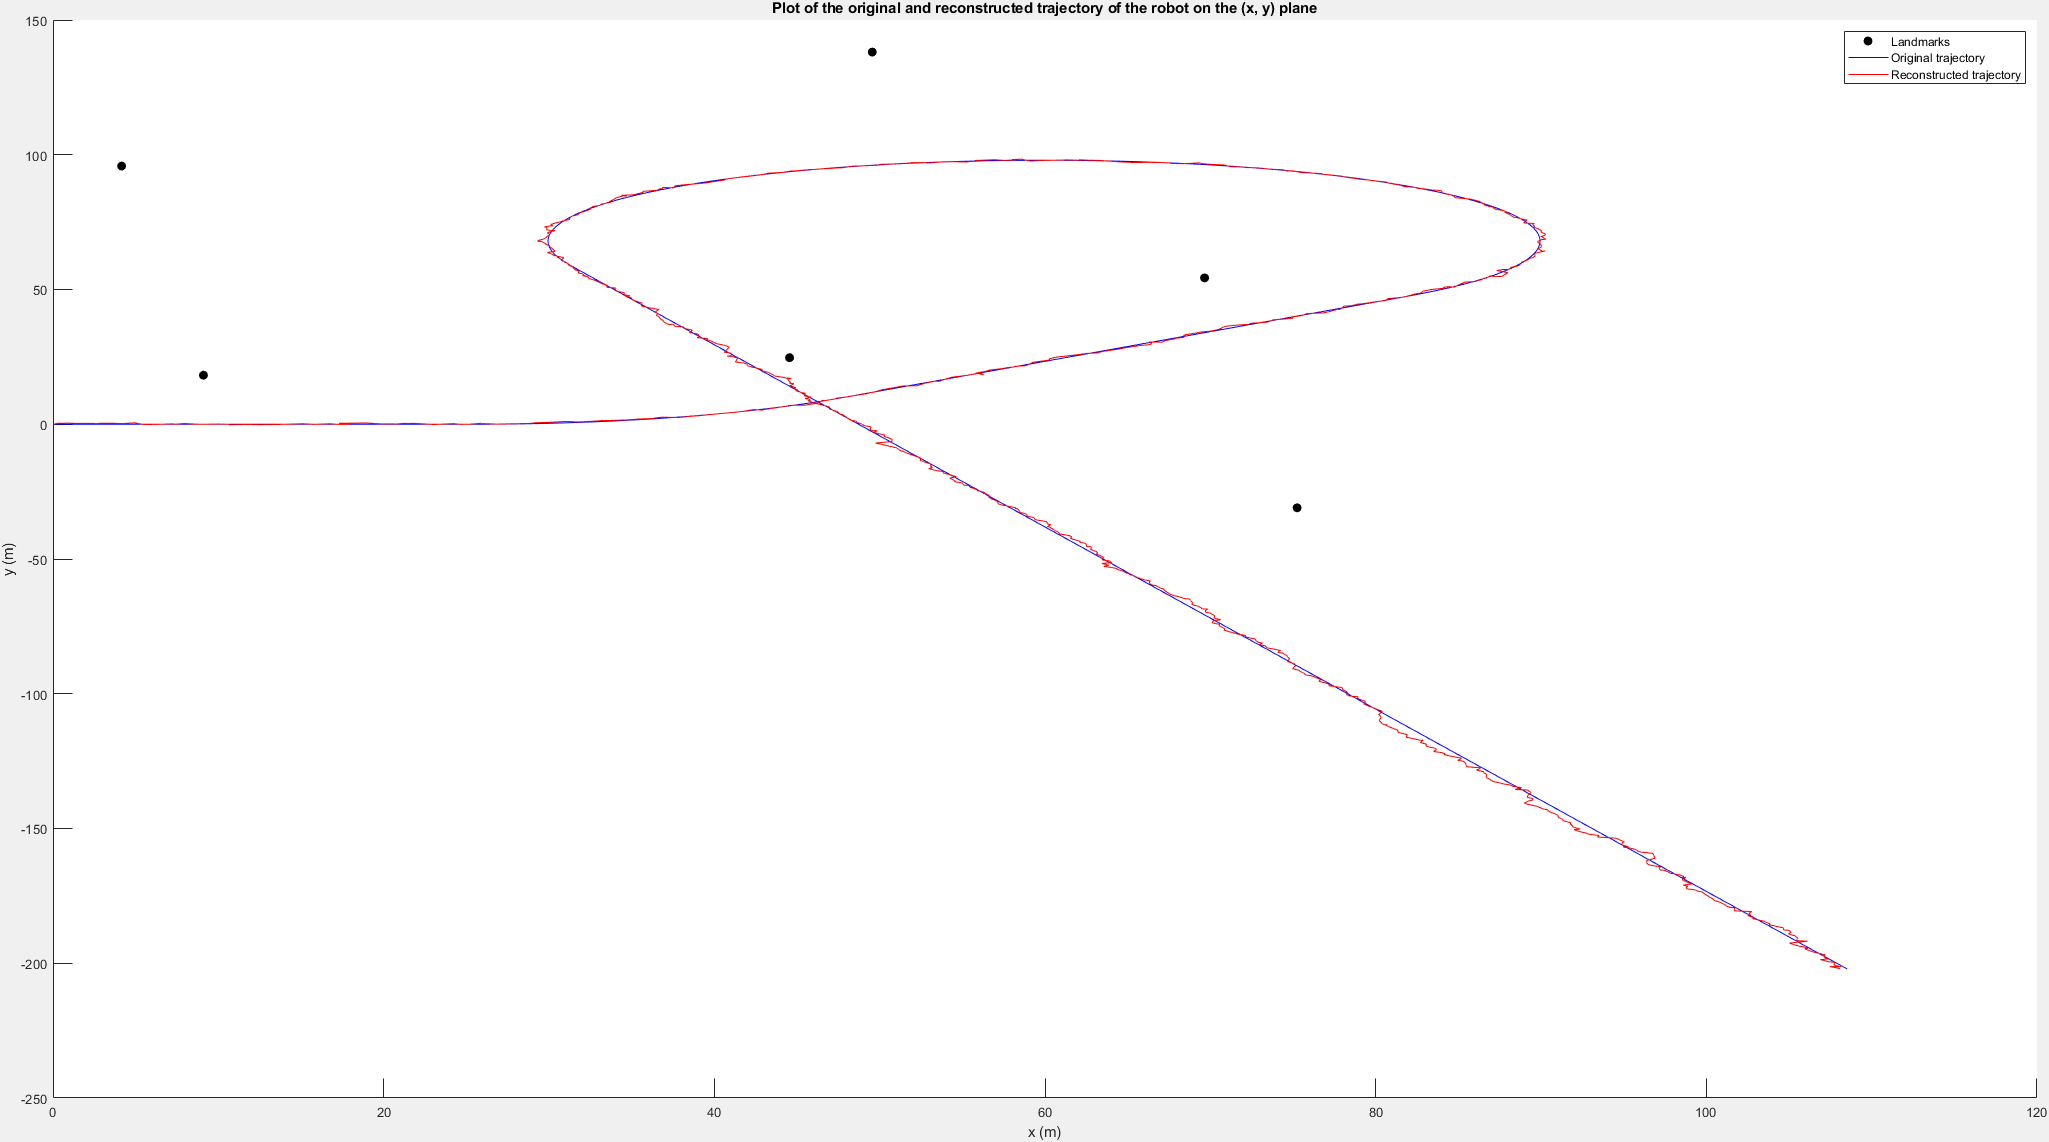
\includegraphics[width=\columnwidth]{images/EKF_trajectory.png}
    \caption{Original and reconstructed trajectory by EKF.}
    \label{fig:EKF_trajectory}
\end{figure}
% Subplots
\begin{figure}
    \centering
    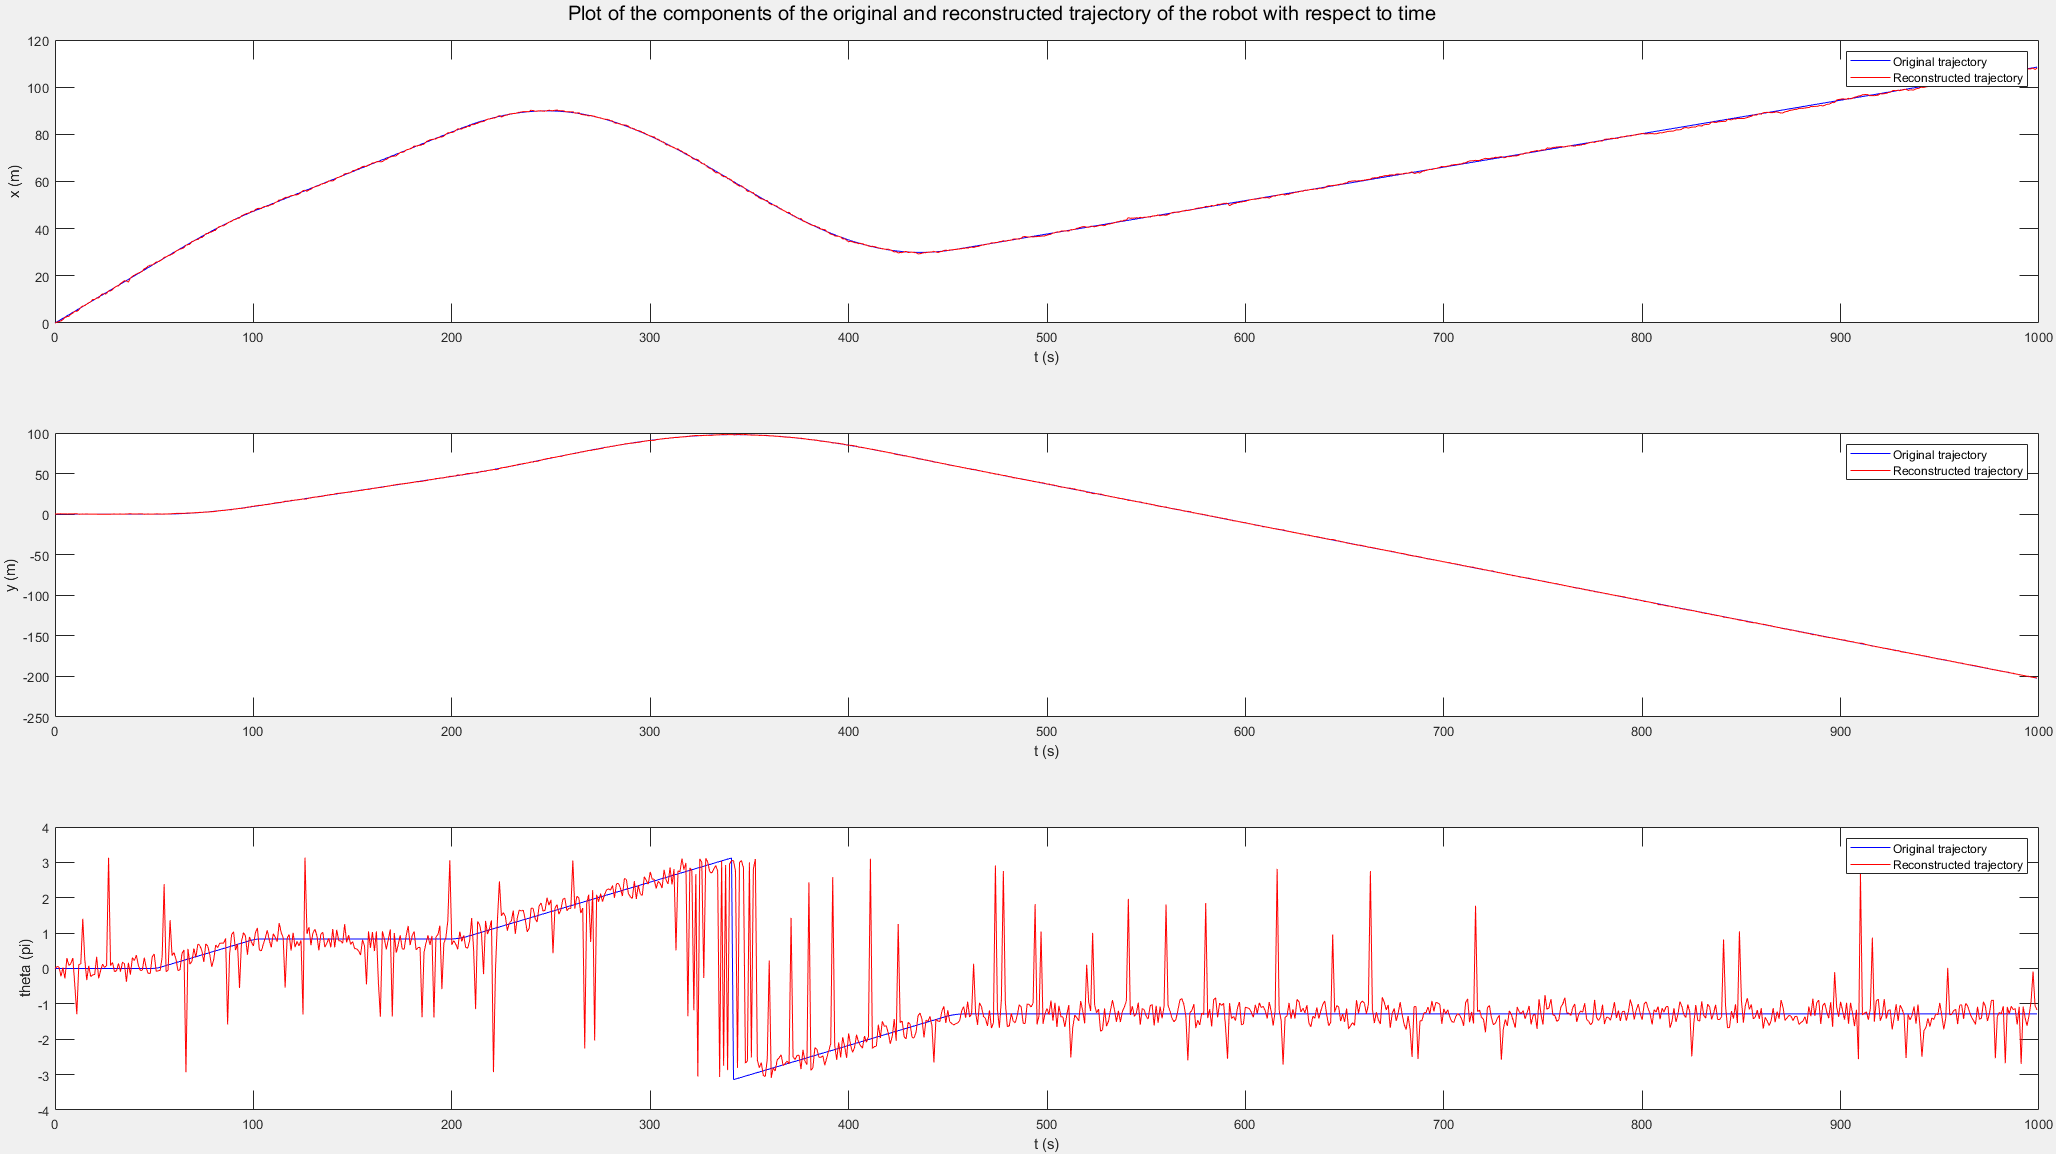
\includegraphics[width=\columnwidth]{images/EKF_subplot.png}
    \caption{Original and reconstructed trajectory components with respect to time by EKF.}
    \label{fig:EKF_subplot}
\end{figure}

%------------------------------------------------------------------------------------------

\subsection{Particle Filter}
The execution time for the particle filter with some example number of particles is shown in Table.\:\ref{tab:execution_time}.
% Compare the results of using 100, 500, 1000 and 3000 particles, report the execution time for each particle set.
\begin{table}
    \centering
    \begin{tabular}{c|c|c|c|c}
        Particles          & $100$      & $500$         & $1000$        & $3000$        \\ 
        \hline
        Execution time (s) & $3.0541$   & $16.2611$     & $31.4827$     & $95.6879$
    \end{tabular}
    \caption{Execution time for particle filter for some example number of particles.}
    \label{tab:execution_time}
\end{table}
Fig.\:\ref{fig:pf_trajectory} shows the trajectory for the particle filter and Fig.\:\ref{fig:pf_subplot} shows the trajectory components as functions of time when using $3000$ particles, both figures containing original trajectory for reference.
% Trajectory
\begin{figure}
    \centering
    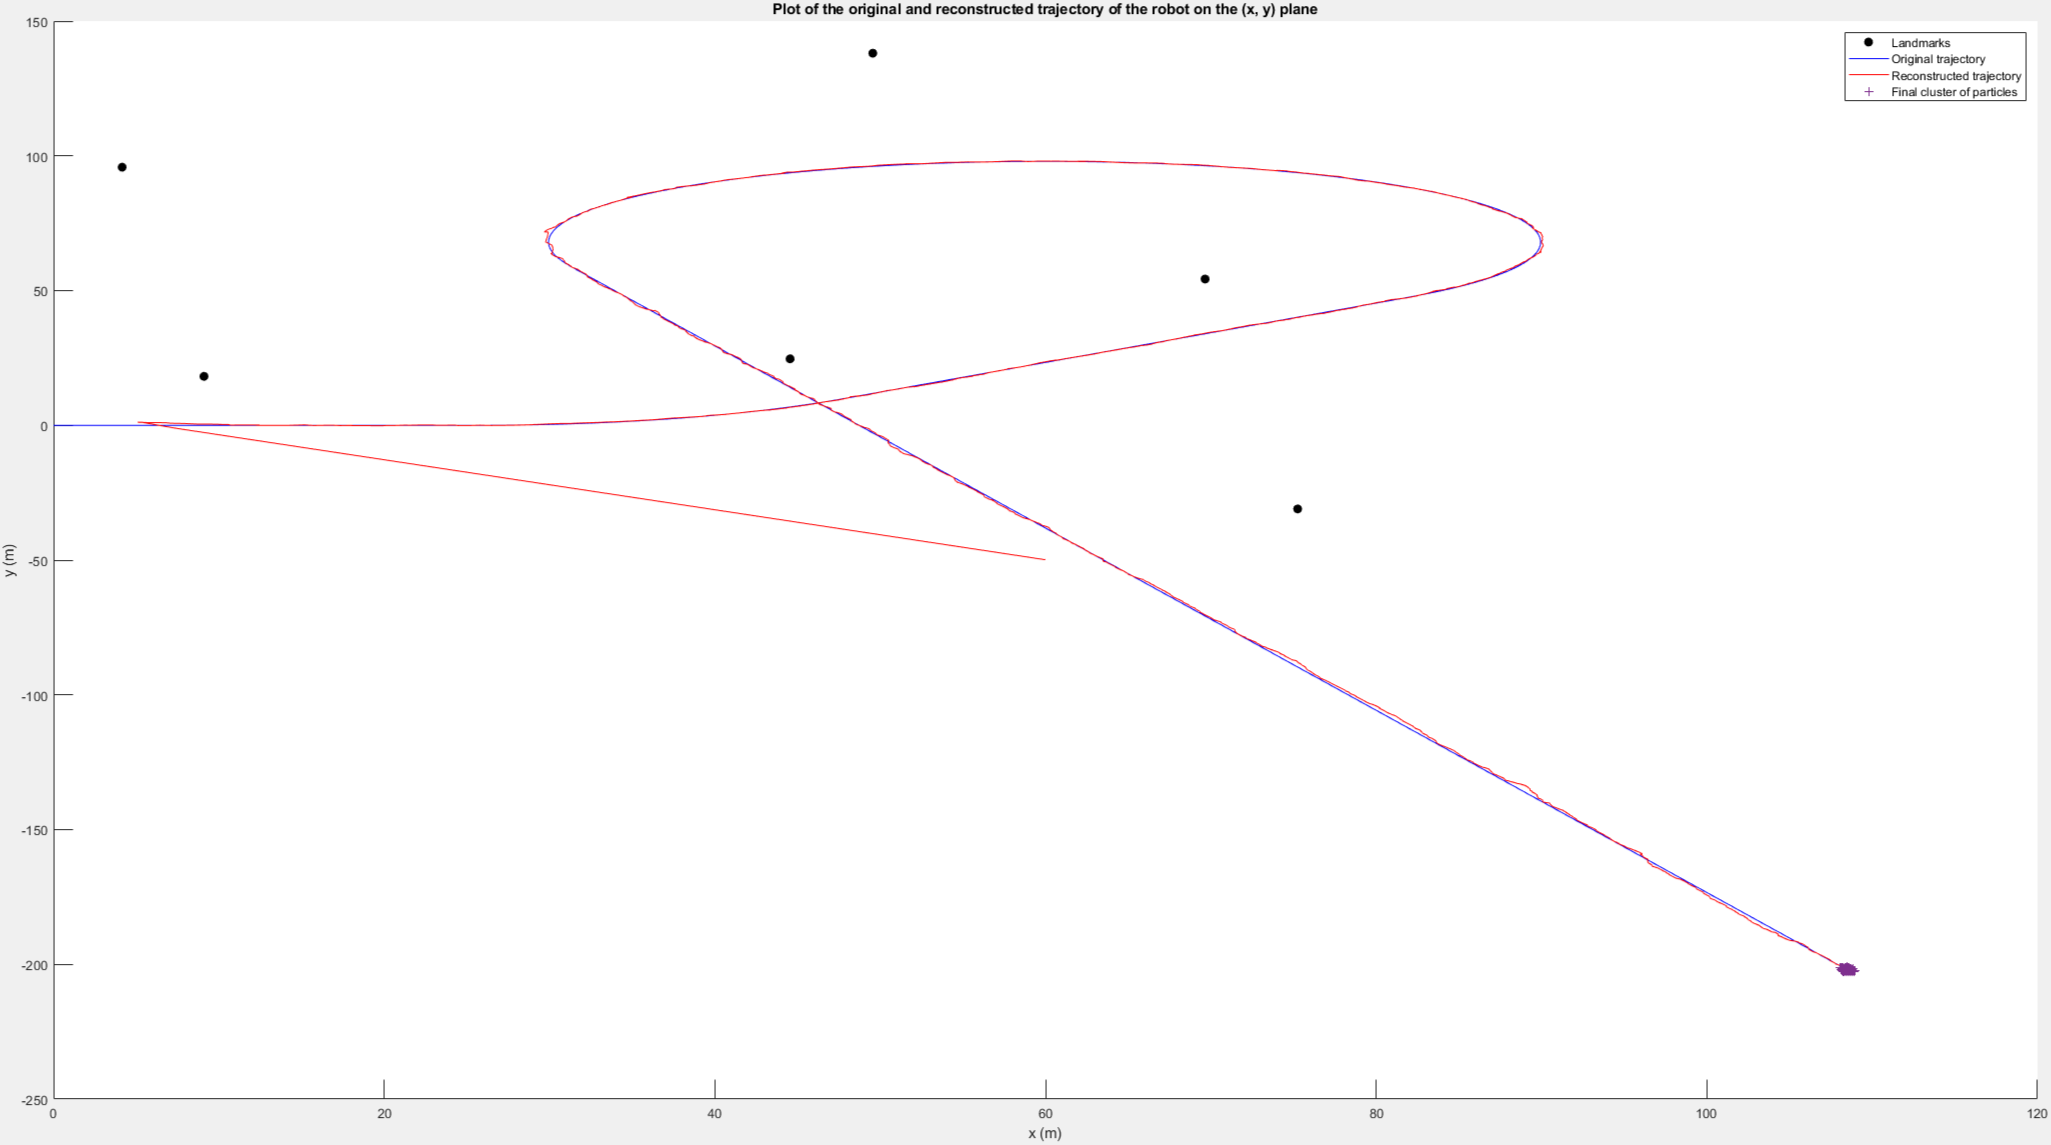
\includegraphics[width=\columnwidth]{images/pf_trajectory.png}
    \caption{Particle filter reconstructed trajectory using 3000 particles and original trajectory.}
    \label{fig:pf_trajectory}
\end{figure}
% Subplots
\begin{figure}
    \centering
    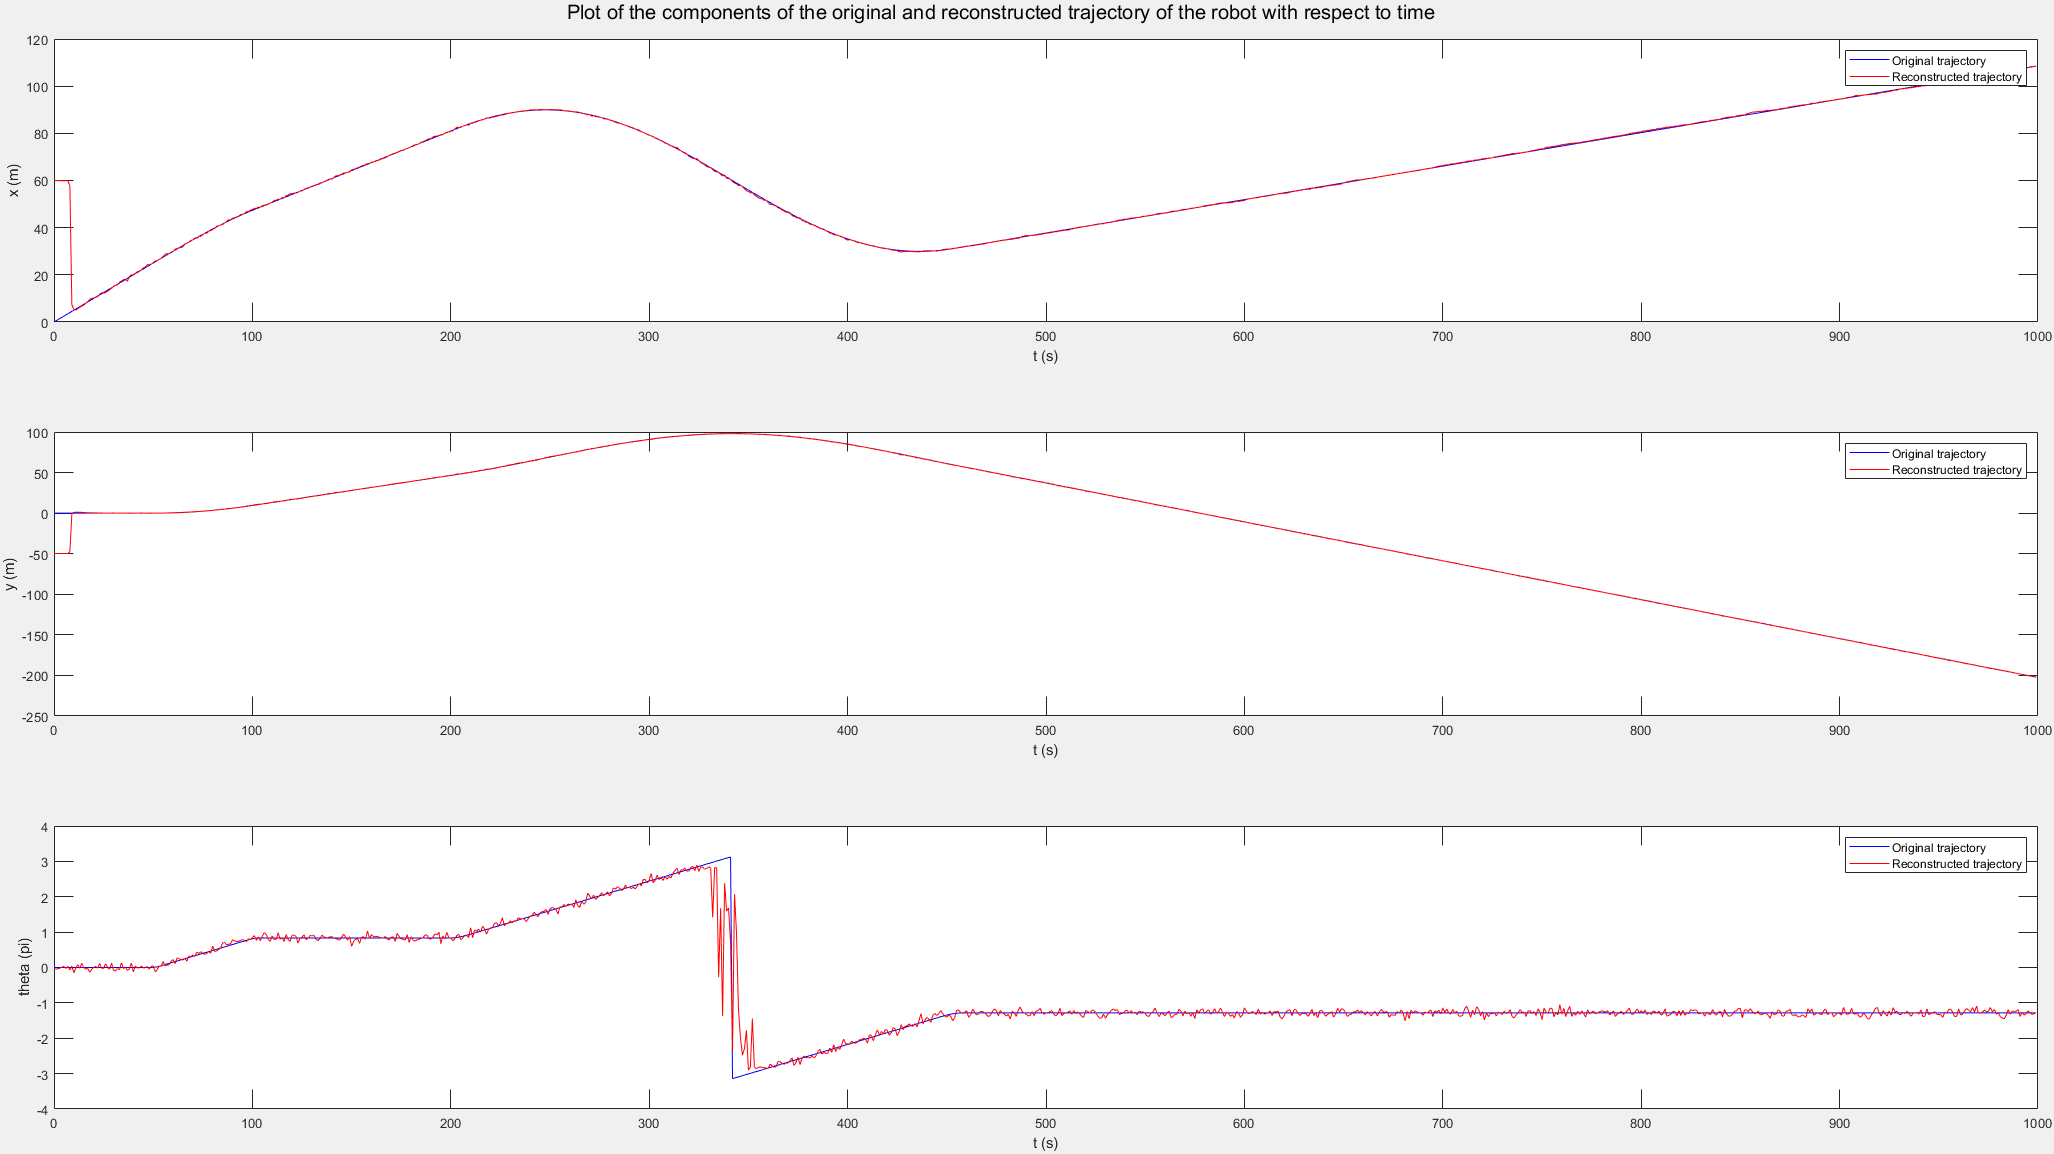
\includegraphics[width=\columnwidth]{images/pf_subplot.png}
    \caption{Particle filter reconstructed trajectory components as a function of time using 3000 particles, with original trajectory for reference.}
    \label{fig:pf_subplot}
\end{figure}

%------------------------------------------------------------------------------------------


%------------------------------------------------------------------------------------------
\begin{comment}
    
\end{comment}
%------------------------------------------------------------------------------------------